\chapter{Độ bội, entropy và cân bằng có ràng buộc}

\lectureoverview{Một phân bố xác suất trở thành một đối tượng nhiệt động lực học
khi các trạng thái của nó mang năng lượng. Trước hết, ta liên hệ sự tăng
entropy với quá trình đạt cân bằng và dùng \(dE=T\,dS\) để suy ra chiều truyền
nhiệt. Sau đó, ta thay một hệ bằng một tập hợp lớn các bản sao, đếm các cách
sắp xếp gắn với mỗi bộ số chiếm chỗ, và chỉ ra rằng logarit của độ bội này
bằng \(N\) lần entropy. Vì vậy, cân bằng là một bài toán cực đại entropy
có ràng buộc. Các nhân tử Lagrange cung cấp phương pháp cần thiết để giải
nó.}

\section{Ba đại lượng cơ bản}

Cho \(i\) làm nhãn cho các trạng thái rời rạc mà một hệ có thể có. Hiện
thời, tính rời rạc hữu ích vì nó cho phép ta đếm trạng thái mà không phải đưa
vào các độ đo không gian pha. Nếu xác suất của trạng thái \(i\) là
\(P_i\), thì
\begin{equation}
 \sum_i P_i=1.
 \label{eq:sm3-normalization}
\end{equation}
Nếu năng lượng của trạng thái đó là \(E_i\), thì năng lượng trung bình là
\begin{equation}
 \overline E=\sum_iP_iE_i.
 \label{eq:sm3-mean-energy}
\end{equation}
Chữ \emph{trung bình} rất quan trọng. Hệ không nhất thiết phải có
giá trị \(\overline E\) trong bất kỳ vi trạng thái nào; đó là giá trị trung bình có
trọng số xác suất trên các giá trị có thể có.

\begin{classroomqa}
\classquestion{Ở đây có sự phân biệt hữu ích nào giữa xác suất và
thống kê không?}
\lecturerresponse{Xác suất cung cấp một mô hình cho các kết quả có thể xảy ra, còn
thống kê thường bắt đầu từ dữ liệu quan sát được rồi hỏi có thể suy ra điều
gì từ đó. Phép tính hiện tại dùng các phân bố xác suất, mặc dù chính những
giá trị trung bình ấy cũng xuất hiện một cách tự nhiên trong dữ liệu thống
kê. Cuộc trao đổi không chính thức trên lớp dùng hai từ này khá linh hoạt vì
sự phân biệt đó không ảnh hưởng đến phần vật lý tiếp theo.
\lecturetimestamp{00:01:39--00:02:21}}
\end{classroomqa}

Entropy của phân bố là
\begin{equation}
 S[P]=-\sum_iP_i\log P_i.
 \label{eq:sm3-entropy}
\end{equation}
Biểu thức này không âm. Mọi xác suất khác không đều thỏa mãn
\(0<P_i\leq1\), nên \(\log P_i\leq0\), và giá trị giới hạn quy ước
\(P_i\log P_i\to0\) được áp dụng khi \(P_i\to0\).

\begin{figure}[t]
\centering
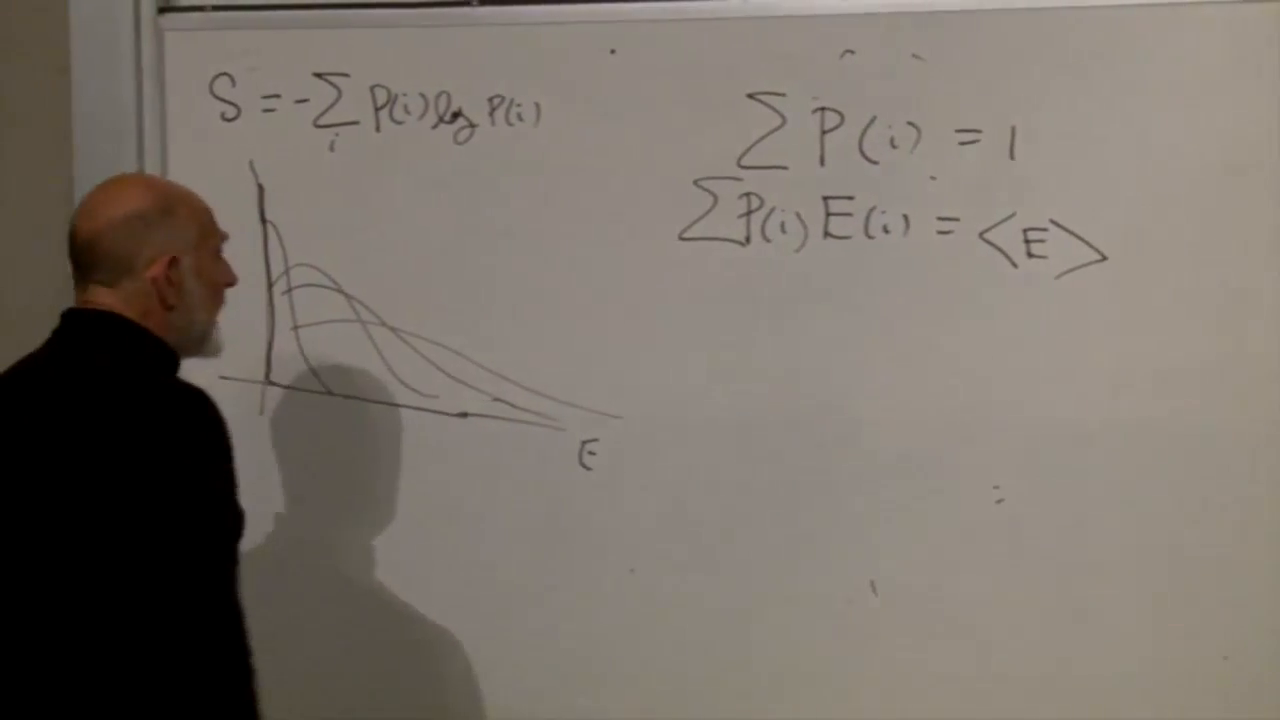
\includegraphics[width=0.88\textwidth]{lecture_03_figure_02.png}
\caption{Bảng mở đầu tập hợp các công thức entropy, chuẩn hóa và năng lượng
trung bình, cùng với một họ định tính các phân bố cân bằng.}
\lectureframe{00:06:44}
\end{figure}

\section{Cân bằng như một họ phân bố}

Bài giảng trước để lại cho ta một họ một tham số các phân bố cân bằng. Có
thể gán nhãn cho họ ấy bằng nhiệt độ, nhưng hiện giờ gán nhãn bằng năng lượng
trung bình \(\overline E\) hữu ích hơn. Ở mức năng lượng nhỏ nhất có thể, phân bố
tập trung vào một trạng thái cơ bản:
\[
 P_i=\delta_{i0}.
\]
Khi đó không còn bất định nào về trạng thái, và \(S=0\). Khi phân bố
cân bằng trải ra trên nhiều mức năng lượng hơn, cả năng lượng trung bình lẫn
entropy của nó đều tăng.

Đây là phát biểu về họ phân bố nhiệt, chứ không phải về mọi phân bố có thể
nghĩ ra. Một họ tùy ý có thể dịch về phía năng lượng lớn hơn đồng thời trở
nên hẹp hơn. Các phân bố cân bằng mà ta sắp suy ra không hành xử như vậy
trong miền nhiệt độ dương thông thường. Dọc theo họ đó,
\begin{equation}
 \frac{dS}{d\overline E}>0.
 \label{eq:sm3-positive-temperature-branch}
\end{equation}
Các hệ có phổ bị chặn cũng có thể có những nhánh mà trên đó đạo hàm này âm.
Những miền nhiệt độ âm đó là có thật, nhưng chúng được tạm gác sang một bên
trong lập luận này.

Cân bằng nhiệt có ý nghĩa nhiều hơn là sự đứng yên ở mức vi mô. Các phân tử
vẫn tiếp tục chuyển động, va chạm và trao đổi năng lượng. Điều trở nên dừng
theo thời gian là mô tả vĩ mô: phân bố không còn biểu lộ một độ trôi ròng,
và các phần tách biệt của hệ không còn duy trì một dòng năng lượng ròng.

\section{Các định luật nhiệt động lực học bằng ngôn ngữ thống kê}

Định luật thứ nhất là sự bảo toàn năng lượng. Định luật thứ hai phát biểu
rằng entropy nhiệt động lực học của một hệ vĩ mô cô lập không giảm:
\begin{equation}
 \Delta S_{\mathrm{tot}}\geq0.
 \label{eq:sm3-second-law}
\end{equation}
Dấu bằng mô tả trạng thái cân bằng hoặc một biến đổi thuận nghịch lý tưởng;
một quá trình thư giãn tự phát thông thường cho một sự tăng nghiêm ngặt.

Trong bức tranh xác suất, quá trình thư giãn có xu hướng phân tán trọng số
xác suất trên các khả năng vĩ mô mà ta vẫn còn phân biệt được. Phát biểu này
cần kèm theo sự lưu ý được nhấn mạnh trong bài giảng: ta đang \emph{làm thô}.
Sự tiến hóa Hamilton chính xác bảo toàn entropy hạt mịn của không gian pha.
Entropy vĩ mô tăng vì ta không còn theo dõi các tương quan và chi tiết vi mô.
Việc mất đi thông tin như vậy làm mô tả rút gọn rộng ra. Trái lại, một sự thu
hẹp tự phát sẽ có nghĩa là ta đã thu được thông tin vi mô mà không thực hiện
phép đo.

Định luật thứ không khẳng định rằng các hệ có thể đạt cân bằng nhiệt và rằng
trạng thái cân bằng có tính bắc cầu. Nếu \(A\) cân bằng với \(B\), và \(B\)
cân bằng với \(C\), thì \(A\) cân bằng với \(C\). Nhiệt độ cung cấp đại
lượng số làm cho tính bắc cầu này trở nên hiển nhiên:
\[
 T_A=T_B,\qquad T_B=T_C
 \quad\Longrightarrow\quad
 T_A=T_C.
\]
Khi chưa cân bằng, năng lượng truyền từ phân hệ có nhiệt độ lớn hơn sang
phân hệ có nhiệt độ nhỏ hơn. Khi nhiệt độ bằng nhau, dòng ròng chấm dứt. Bây
giờ ta suy ra phát biểu thao tác đó từ định nghĩa entropy của nhiệt độ.

\section{Vì sao năng lượng truyền từ nơi nóng sang nơi lạnh}

Xét hai phân hệ ghép yếu \(A\) và \(B\). Mỗi phân hệ đều đang cân
bằng nội bộ, nhưng nhiệt độ của chúng khác nhau. Chọn ký hiệu sao cho
\begin{equation}
 T_B>T_A>0.
 \label{eq:sm3-temperature-order}
\end{equation}
Trong một trao đổi nhỏ, bảo toàn năng lượng của hệ gộp cho
\begin{equation}
 dE_A+dE_B=0.
 \label{eq:sm3-energy-conservation}
\end{equation}
Định luật thứ hai cho
\begin{equation}
 dS_A+dS_B\geq0.
 \label{eq:sm3-entropy-change}
\end{equation}
Đối với mỗi phân hệ đang cân bằng nội bộ, nhiệt độ được định nghĩa bởi
\begin{equation}
 dE_X=T_X\,dS_X,
 \qquad X=A,B.
 \label{eq:sm3-temperature-differential}
\end{equation}
Thế vào \eqref{eq:sm3-energy-conservation}, ta được
\begin{equation}
 T_A\,dS_A+T_B\,dS_B=0,
\end{equation}
và do đó
\begin{equation}
 dS_B=-\frac{T_A}{T_B}\,dS_A.
 \label{eq:sm3-dsb}
\end{equation}
Đưa kết quả này vào \eqref{eq:sm3-entropy-change},
\begin{align}
 dS_{\mathrm{tot}}
 &=dS_A-\frac{T_A}{T_B}dS_A\\
 &=\frac{T_B-T_A}{T_B}\,dS_A\geq0.
 \label{eq:sm3-flow-entropy}
\end{align}
Vì \(T_B-T_A>0\) và \(T_B>0\), một trao đổi tự phát đòi hỏi
\[
 dS_A>0.
\]
Khi đó \eqref{eq:sm3-temperature-differential} cho
\begin{equation}
 dE_A=T_A\,dS_A>0,
 \qquad
 dE_B=-dE_A<0.
 \label{eq:sm3-hot-to-cold}
\end{equation}
Năng lượng đã truyền từ \(B\), phân hệ nóng hơn, sang \(A\), phân hệ
lạnh hơn. Ở đây, nhiệt đơn giản chỉ là năng lượng đang truyền. Dòng truyền
này tiếp tục cho đến khi \(T_A=T_B\), khi đó biến thiên entropy bậc nhất không
còn ưu tiên chiều nào nữa.

Cùng kết quả đó có thể được trình bày trong một dòng:
\begin{equation}
 dS_{\mathrm{tot}}
 =dE_A\left(\frac{1}{T_A}-\frac{1}{T_B}\right)\geq0.
 \label{eq:sm3-compact-flow}
\end{equation}
Dấu của hiệu nghịch đảo nhiệt độ quyết định dấu của \(dE_A\). Dạng gọn này
về sau sẽ phù hợp tự nhiên với tập hợp chính tắc.

\begin{classroomqa}
\audiencequestion{Lập luận này có giả thiết rằng \(A\) và \(B\) mỗi phân hệ đều đã
ở cân bằng nội bộ không?}
\lecturerresponse{Có. Việc gán một \(T_A\) hay \(T_B\) duy nhất đã bao hàm giả thiết
đó. Nếu một phân hệ chưa cân bằng nội bộ, hãy chia nó thành các vùng nhỏ hơn
và áp dụng lập luận này cục bộ ở bất cứ nơi nào có thể định nghĩa nhiệt độ.
Khi đó, quá trình thư giãn toàn cục được ghép lại từ các trao đổi giữa những
vùng ấy.
\lecturetimestamp{00:24:38--00:25:22}}
\end{classroomqa}

\section{Thế nào được coi là một trạng thái?}

Trước khi hỏi các xác suất cân bằng là gì, ta phải biết nhãn \(i\) có
nghĩa gì. Một trạng thái vi mô là mô tả đầy đủ nhất về hệ mà các định luật
vật lý cơ bản cho phép. Trong cơ học cổ điển, ta hình dung đó là các vị trí
và động lượng của mọi hạt. Trong cơ học lượng tử, thay vào đó, một trạng thái
là một trạng thái lượng tử đầy đủ; nguyên lý bất định ngăn cản việc xác định
sắc nét đồng thời mọi vị trí và động lượng cổ điển.

Đối với một hệ lượng tử trong một hộp hữu hạn, phép đếm trạng thái thích
hợp có thể là rời rạc. Cơ học thống kê cổ điển xuất hiện trong một giới hạn
thích hợp, nơi các tổng trên các trạng thái lượng tử sít nhau trở thành các
tích phân không gian pha. Quá trình lấy giới hạn đó cũng đưa vào ô không gian
pha cần thiết để làm cho entropy liên tục trở thành vô thứ nguyên; nó không
thu được chỉ bằng cách thay một dấu tổng bằng một dấu tích phân.

\begin{classroomqa}
\audiencequestion{Đối với một chất khí, có nên hình dung một trạng thái là vị trí và
động lượng của mọi phân tử không?}
\lecturerresponse{Đó là bức tranh cổ điển đúng. Tổng quát hơn, một trạng thái có nghĩa
là toàn bộ những gì về nguyên tắc có thể biết về hệ, phù hợp với các định
luật vật lý. Cơ học lượng tử làm thay đổi dạng của mô tả cực đại đó và khiến
phép đếm trong thể tích hữu hạn trở nên rời rạc. Việc khôi phục tích phân cổ
điển từ tổng lượng tử là một lập luận giới hạn thực sự, không phải một phép
thay thế trong một dòng.
\lecturetimestamp{00:25:31--00:27:38}}
\end{classroomqa}

\section{Một bể nhiệt tạo từ các bản sao}

Câu hỏi khó giờ đây không thể tránh khỏi: sau khi cân bằng đã được thiết
lập, điều gì quyết định \(P_i\)?

Đặt phân hệ tiếp xúc với một bể nhiệt rất lớn. Năng lượng có thể truyền qua
lại, nhưng bể có quá nhiều bậc tự do đến mức việc truyền một lượng năng lượng
nhỏ hầu như không làm thay đổi nhiệt độ của nó. Một bể đặc biệt thuận tiện
được tạo bởi nhiều bản sao ghép yếu của chính phân hệ đó. Một bản sao là hệ
đang được nghiên cứu; các bản sao còn lại cấu thành môi trường của nó.

Cách xây dựng này thường phản ánh một hệ vĩ mô thực. Hãy chia một vật thể
lớn gần như đồng nhất thành nhiều ô tương tự nhau. Mỗi ô là một phân hệ, còn
các ô còn lại đóng vai trò bể nhiệt của nó. Ký hiệu tổng số bản sao là \(N\).
Minh họa trên lớp dùng chín bản sao và ba nhãn trạng thái tô màu, nhưng phép
đếm không phụ thuộc vào những con số cụ thể đó.

Gọi \(n_i\) là số bản sao ở trạng thái \(i\). Đây là các
\emph{số chiếm đóng}. Có thể có vô hạn mức năng lượng khả dĩ, nhưng với tổng năng lượng hữu hạn thì phần lớn các mức rất cao có độ chiếm đóng không đáng kể hoặc bằng không.

Ràng buộc thứ nhất đơn giản là số bản sao:
\begin{equation}
 \sum_i n_i=N.
 \label{eq:sm3-number-constraint}
\end{equation}
Ràng buộc thứ hai là tổng năng lượng:
\begin{equation}
 \sum_i n_iE_i=N\overline E.
 \label{eq:sm3-total-energy-constraint}
\end{equation}
Vế phải là đại lượng quảng tính. Nếu số bản sao được nhân đôi trong khi trạng thái thống kê của chúng được giữ cố định, thì tổng năng lượng tăng gấp đôi, còn năng lượng trung bình trên mỗi bản sao vẫn là \(\overline E\).

\begin{classroomqa}
\audiencequestion{Việc xây dựng bằng bản sao có nhất thiết cũng phải thỏa một ràng buộc năng lượng không?}
\lecturerresponse{Có. Các số chiếm đóng phải cộng lại thành \(N\), và tổng có trọng số theo năng lượng của chúng phải bằng tổng năng lượng cố định \(N\overline E\).
Đó chính xác là hai ràng buộc mà về sau sẽ giới hạn cực đại entropy.
\lecturetimestamp{00:37:12--00:39:54}}
\end{classroomqa}

Xác suất để một bản sao được chọn ngẫu nhiên ở trạng thái \(i\) chính là tần suất tương đối của nó:
\begin{equation}
 P_i=\frac{n_i}{N},
 \qquad
 n_i=NP_i.
 \label{eq:sm3-frequency-probability}
\end{equation}

\begin{figure}[t]
\centering
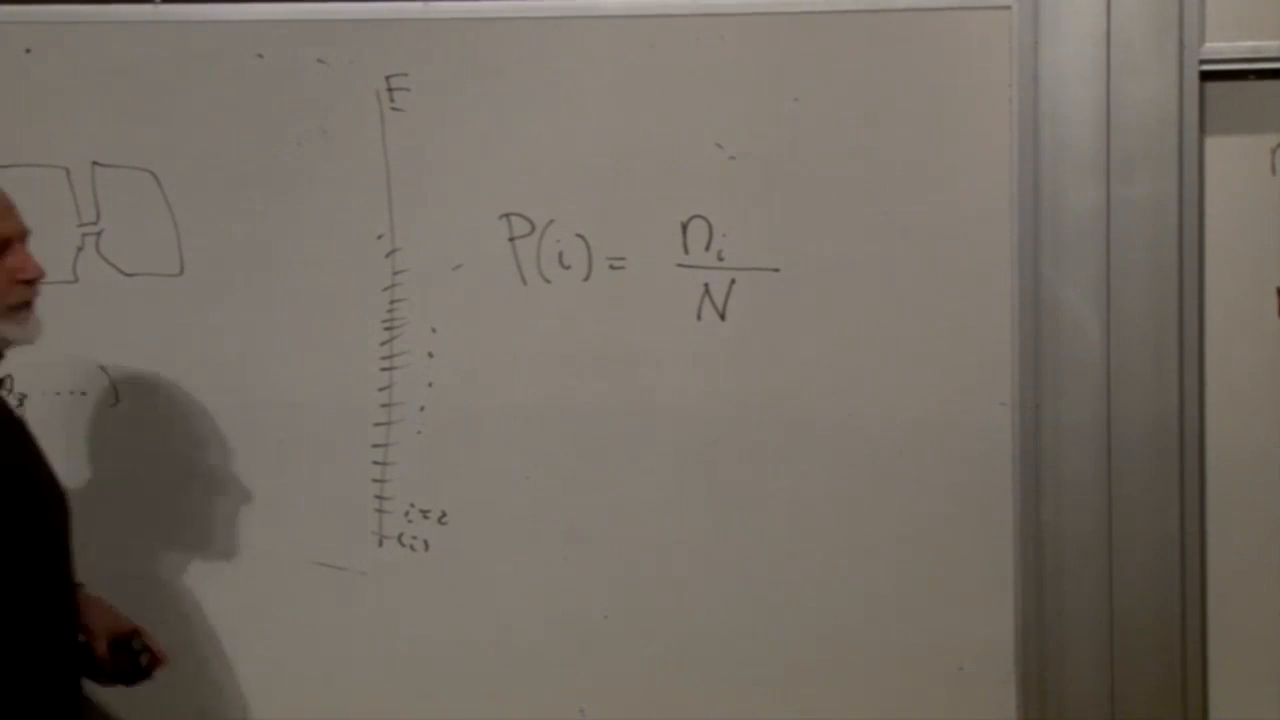
\includegraphics[width=0.82\textwidth]{lecture_03_figure_03.png}
\caption{Bức tranh mức năng lượng và việc đồng nhất xác suất với phần chiếm đóng \(P_i=n_i/N\).}
\lectureframe{00:41:40}
\end{figure}

\begin{classroomqa}
\audiencequestion{Ký hiệu \(N(i)\) trên bảng có được dùng với ý nghĩa khác \(n_i\) không?}
\lecturerresponse{Không. Cả hai đều ký hiệu số chiếm đóng của trạng thái \(i\). Ta dùng \(n_i\) một cách nhất quán và dành chữ hoa \(N\) cho tổng số bản sao.
\lecturetimestamp{00:41:28--00:41:33}}
\end{classroomqa}

Chia \eqref{eq:sm3-number-constraint} và
\eqref{eq:sm3-total-energy-constraint} cho \(N\) sẽ thu lại các ràng buộc xác suất:
\begin{equation}
 \sum_iP_i=1,
 \qquad
 \sum_iP_iE_i=\overline E.
 \label{eq:sm3-probability-constraints}
\end{equation}
Vì vậy, cách diễn giải xác suất theo tần suất trong ensemble đã tái tạo lại các phương trình mà ta đã bắt đầu.

\section{Độ bội của một mẫu chiếm đóng}

Cố định một tập số chiếm đóng \(\{n_i\}\). Có bao nhiêu cách phân các
\(N\) bản sao phân biệt được vào các trạng thái để thực hiện đúng tập ấy? Câu trả lời là hệ số đa thức
\begin{equation}
 C(\{n_i\})=\frac{N!}{\prod_i n_i!}.
 \label{eq:sm3-multiplicity}
\end{equation}
Để thấy được mẫu số, trước hết hãy sắp xếp tất cả \(N\) bản sao có nhãn theo \(N!\) thứ tự. Hoán vị các \(n_i\) bản sao chiếm cùng một trạng thái không tạo ra một cách phân bố chiếm đóng mới, nên phải chia cho \(n_i!\) đối với mỗi trạng thái.

\begin{figure}[t]
\centering
\includegraphics[width=0.88\textwidth]{lecture_03_figure_04.png}
\caption{Độ bội đa thức
\(C=N!/\prod_i n_i!\) được viết trên bảng.}
\lectureframe{00:46:55}
\end{figure}

Các mức không bị chiếm không gây vấn đề gì vì \(0!=1\). Nếu tất cả các bản sao đều chiếm một trạng thái, thì
\[
 C=\frac{N!}{N!}=1,
\]
đúng như dự kiến. Nếu ba bản sao chiếm ba trạng thái xác định khác nhau, thì
\[
 C=\frac{3!}{1!\,1!\,1!}=6.
\]
Với hai bản sao chiếm hai trạng thái xác định, công thức cho hai cách gán: hoán đổi bản sao có nhãn nào chiếm trạng thái nào.

\begin{classroomqa}
\audiencequestion{Có thể có hơn một tập số chiếm đóng thỏa hai ràng buộc không?}
\lecturerresponse{Thường thì có nhiều tập như vậy. Phương trình
\eqref{eq:sm3-multiplicity} trước hết đếm số cách sắp xếp cho một tập cố định
\(\{n_i\}\), mà chưa quyết định liệu nó có thỏa các ràng buộc hay không. Bước tiếp theo so sánh mọi tập tương thích với các ràng buộc và tìm tập nào có độ bội lớn nhất.
\lecturetimestamp{00:48:07--00:48:43}}
\end{classroomqa}

Giả thiết thống kê là các cách gán vi mô tương thích với cách bố trí cô lập được xử lý đối xứng. Vì thế, một mẫu chiếm đóng vĩ mô được thực hiện bởi nhiều cách gán hơn sẽ có xác suất lớn hơn. Với \(N\) lớn, phân bố theo các tỉ phần \(n_i/N\) trở nên nhọn rõ rệt. Các tỉ phần cân bằng là những giá trị làm cực đại \(C\), với các ràng buộc \eqref{eq:sm3-number-constraint} và
\eqref{eq:sm3-total-energy-constraint}.

\section{Xấp xỉ Stirling}

Các giai thừa trở nên khổng lồ từ rất lâu trước khi \(N\) đạt tới một giá trị vĩ mô, nên ta làm việc với logarit của chúng. Bắt đầu từ
\begin{equation}
 \log N!=\sum_{x=1}^{N}\log x.
 \label{eq:sm3-log-factorial-sum}
\end{equation}
Với \(N\) lớn, tổng được xấp xỉ bằng diện tích dưới \(\log x\):
\begin{align}
 \log N!
 &\simeq\int_1^N\log x\,dx\\
 &=\left[x\log x-x\right]_1^N\\
 &=N\log N-N+1.
 \label{eq:sm3-stirling-integral}
\end{align}
Nguyên hàm suy ra ngay từ
\[
 \frac{d}{dx}(x\log x-x)=\log x.
\]
Ở bậc quảng tính dẫn đầu, có thể bỏ hằng số cộng:
\begin{equation}
 \log N!\simeq N\log N-N.
 \label{eq:sm3-stirling-log}
\end{equation}
Lấy mũ cho ta dạng đơn giản được dùng trong bài giảng,
\begin{equation}
 N!\simeq N^N e^{-N}.
 \label{eq:sm3-stirling-simple}
\end{equation}

\begin{figure}[t]
\centering
\includegraphics[width=0.88\textwidth]{lecture_03_figure_05.png}
\caption{Xấp xỉ Stirling bậc dẫn đầu và phép suy ra nó bằng cách thay
tổng của \(\log x\) bằng một tích phân.}
\lectureframe{01:03:45}
\end{figure}

\begin{classroomqa}
\audiencequestion{Khi tính \(x\log x-x\) tại cận dưới, có xuất hiện thêm
\(+1\) không?}
\lecturerresponse{Có. Phương trình \eqref{eq:sm3-stirling-integral} có chứa
hằng số đó. Nó không đáng kể so với các số hạng tỉ lệ với \(N\) khi
\(N\to\infty\), đó là lý do công thức bậc dẫn đầu bỏ nó đi. Bản thân tổng
phải bắt đầu tại \(x=1\); \(\log0\) không xác định.
\lecturetimestamp{01:04:12--01:04:35}}
\end{classroomqa}

\begin{classroomqa}
\audiencequestion{Có phải cũng còn thiếu một thừa số tỉ lệ với \(\sqrt{N}\) không?}
\lecturerresponse{Có. Công thức tiệm cận sắc hơn là
\[
 N!\sim\sqrt{2\pi N}\left(\frac{N}{e}\right)^N.
\]
Logarit của nó chỉ thêm \(\tfrac12\log(2\pi N)\), là dưới quảng tính
so với \(N\log N-N\). Nó quan trọng đối với các xác suất chính xác khi \(N\)
 hữu hạn, nhưng không quan trọng đối với phép tính entropy bậc dẫn đầu của một hệ vĩ mô.
\lecturetimestamp{01:04:35--01:05:40}}
\end{classroomqa}

Xấp xỉ Stirling cũng phải được dùng cẩn trọng ở mẫu số của
\eqref{eq:sm3-multiplicity}. Trong giới hạn nhiệt động, các trạng thái mang
xác suất giới hạn khác không có \(n_i=NP_i\), nên số chiếm đóng của chúng tăng
cùng \(N\). Các trạng thái có độ chiếm đóng rất nhỏ hoặc triệt tiêu có thể được xử lý bằng một ngưỡng cắt năng lượng hữu hạn rồi khôi phục bằng một phép lấy giới hạn. Entropy quảng tính bậc dẫn đầu không bị ảnh hưởng bởi các số hạng dưới dẫn đầu đã lược bỏ.

\section{Logarit của độ bội là entropy}

Áp dụng \eqref{eq:sm3-stirling-simple} cho tử số và mọi thừa số ở mẫu có
chiếm đóng vĩ mô:
\begin{equation}
 C\simeq
 \frac{N^Ne^{-N}}
 {\prod_i n_i^{\,n_i}e^{-n_i}}.
 \label{eq:sm3-c-stirling}
\end{equation}
Vì \(\sum_i n_i=N\), các thừa số mũ bậc dẫn đầu triệt tiêu nhau:
\begin{equation}
 C\simeq\frac{N^N}{\prod_i n_i^{\,n_i}}.
 \label{eq:sm3-c-leading}
\end{equation}
Cực đại hóa logarit dễ hơn cực đại hóa một tích, và logarit là
đơn điệu, nên cả hai cực đại xuất hiện tại cùng một mẫu chiếm đóng:
\begin{equation}
 \log C=N\log N-\sum_i n_i\log n_i.
 \label{eq:sm3-logc-occupations}
\end{equation}
Bây giờ thay \(n_i=NP_i\):
\begin{align}
 \log C
 &=N\log N-\sum_iNP_i\log(NP_i)\\
 &=N\log N-N\sum_iP_i\log N
   -N\sum_iP_i\log P_i\\
 &=-N\sum_iP_i\log P_i,
 \label{eq:sm3-logc-entropy-derivation}
\end{align}
trong đó điều kiện chuẩn hóa làm triệt tiêu hai số hạng \(N\log N\). Do đó, ở bậc dẫn đầu theo \(N\),
\begin{equation}
 \boxed{\log C=NS}.
 \label{eq:sm3-logc-ns}
\end{equation}

\begin{figure}[t]
\centering
\includegraphics[width=0.88\textwidth]{lecture_03_figure_06.png}
\caption{Phép tính trên bảng nối
\(\log C=N\log N-\sum_i n_i\log n_i\) với
\(-N\sum_iP_i\log P_i=NS\).}
\lectureframe{01:16:10}
\end{figure}

Quan hệ này là trung tâm khái niệm của chương. Entropy không phải là một đại lượng không liên quan được áp đặt lên bài toán đếm. Nó là độ bội trên mỗi bản sao, được đo bằng logarit. Vì vậy, cực đại hóa số cách sắp xếp vi mô, ở bậc dẫn đầu, đồng nhất với cực đại hóa entropy của một bản sao.

\begin{classroomqa}
\audiencequestion{Không phải độ bội sẽ lớn nhất khi mọi số chiếm đóng đều bằng nhau sao?}
\lecturerresponse{Phân bố quả là đồng đều khi không trạng thái nào được phân biệt và chỉ có
\(\sum_i n_i=N\) được áp đặt trên một tập hữu hạn trạng thái. Ràng buộc năng lượng cố định
làm thay đổi câu trả lời vì các giá trị \(E_i\) là khác nhau.
Các số chiếm đóng bằng nhau nói chung không tạo ra năng lượng trung bình đã chỉ định.
\lecturetimestamp{01:17:07--01:18:20}}
\end{classroomqa}

\begin{classroomqa}
\audiencequestion{Chữ hoa \(N\) là lớn, nhưng vì sao có thể áp dụng xấp xỉ Stirling
cho mọi \(n_i\) ở mẫu?}
\lecturerresponse{Đối với mỗi trạng thái có xác suất giới hạn khác không,
\(n_i=NP_i\) tăng tỉ lệ với \(N\). Trước hết có thể giữ lại một miền
năng lượng hữu hạn, lấy giới hạn \(N\) lớn ở đó, rồi sau đó mở rộng miền ấy.
Các trạng thái ở đuôi thưa cần những hiệu chỉnh hữu hạn riêng, nhưng chúng không làm thay đổi
entropy quảng tính bậc dẫn đầu.
\lecturetimestamp{01:18:23--01:19:28}}
\end{classroomqa}

\begin{classroomqa}
\audiencequestion{Xấp xỉ \(N\) lớn này có phải là điều trước đó được hiểu là
làm thô không?}
\lecturerresponse{Không. Giới hạn nhiệt động chi phối các số chiếm đóng lớn
và phép đếm tiệm cận. Làm thô là sự mất đi hoặc sự loại bỏ có chủ ý
độ phân giải vi mô. Chúng là hai thao tác khác nhau, mặc dù cả hai thường được dùng trong cơ học thống kê vĩ mô.
\lecturetimestamp{01:19:29--01:19:46}}
\end{classroomqa}

\begin{classroomqa}
\audiencequestion{Vì
\(\log C=N\log N-\sum_i n_i\log n_i\), có phải số hạng thứ hai nên được cực tiểu hóa
thay vì cực đại hóa không?}
\lecturerresponse{Đúng; khi \(N\) cố định, cực đại hóa \(\log C\) tương đương
với cực tiểu hóa \(\sum_i n_i\log n_i\). Sau khi thay \(n_i=NP_i\), các
số hạng \(N\log N\) cố định triệt tiêu nhau và phần còn lại là
\(-N\sum_iP_i\log P_i=NS\). Vì thế, cùng một thao tác được mô tả tự nhiên
hơn là cực đại hóa entropy dương \(S\).
\lecturetimestamp{01:19:48--01:20:55}}
\end{classroomqa}

\begin{classroomqa}
\audiencequestion{Vì sao không kết thúc lập luận ngay bằng đối xứng và đặt
mọi \(n_i\) bằng nhau?}
\lecturerresponse{Lối tắt đó bỏ qua các nhãn năng lượng. Ràng buộc
chuẩn hóa đối xử các trạng thái một cách đối xứng, nhưng
\(\sum_iP_iE_i=\overline E\) thì không: các trạng thái có năng lượng khác nhau đóng góp
theo những cách khác nhau. Chính trong ràng buộc năng lượng mà phân bố cân bằng không đồng đều xuất hiện.
\lecturetimestamp{01:21:15--01:21:41}}
\end{classroomqa}

\section{Bài toán cực đại entropy}

Giờ đây ta có thể phát biểu quy tắc cơ học thống kê một cách không nhập nhằng. Hãy biến thiên các xác suất \(P_i\) và cực đại hóa
\begin{equation}
 S[P]=-\sum_iP_i\log P_i
 \label{eq:sm3-maximize-entropy}
\end{equation}
với các ràng buộc
\begin{equation}
 \sum_iP_i=1,
 \qquad
 \sum_iP_iE_i=\overline E.
 \label{eq:sm3-maxent-constraints}
\end{equation}
Các xác suất làm cực đại cho ta các tỉ phần chiếm đóng được ưu tiên rõ rệt của một tập hợp lớn các bản sao. Các số chiếm đóng có dao động, nhưng độ lệch tương đối của chúng co lại khi \(N\) tăng, nên các tỉ số \(n_i/N\) trở thành những xác suất nhiệt động lực học được xác định rõ.

\begin{classroomqa}
\audiencequestion{Có phải \(E_i\) là các năng lượng trạng thái cố định, còn ràng buộc thì dùng một tổng năng lượng được cho riêng hay không?}
\lecturerresponse{Đúng. Phổ \(\{E_i\}\) thuộc về hệ con.
Toàn bộ tập hợp các bản sao có một tổng năng lượng cố định, nhưng năng lượng
liên tục chuyển giữa các bản sao. Lấy tổng đó chia cho \(N\) sẽ cố định năng lượng
trung bình \(\overline E\) của một bản sao, chứ không phải năng lượng của nó trong từng hiện thực
vi mô.
\lecturetimestamp{01:26:12--01:27:07}}
\end{classroomqa}

Bài toán thì dễ phát biểu và vẫn chưa được giải. Đây là một bài toán cực trị với hai ràng buộc, nên cần thêm một công cụ toán học nữa.

\section{Các nhân tử Lagrange}

Đối với một hàm không bị ràng buộc \(F(x_1,x_2,\ldots)\), một điểm dừng
thỏa mãn
\begin{equation}
 \frac{\partial F}{\partial x_i}=0
 \qquad\text{for every }i.
 \label{eq:sm3-unconstrained-stationary}
\end{equation}
Bây giờ hãy thêm yêu cầu rằng
\begin{equation}
 G(x_1,x_2,\ldots)=0.
 \label{eq:sm3-one-constraint}
\end{equation}

\begin{classroomqa}
\audiencequestion{Nếu hình vẽ có các tọa độ \(x\)
và \(y\) thì \(x\) có nghĩa là gì?}
\lecturerresponse{Ở đây \(x\) là cách viết tắt cho toàn bộ véc-tơ tọa độ
\((x_1,x_2,\ldots)\). Trong hình vẽ hai chiều, các thành phần của nó
chỉ đơn giản là \(x\) và \(y\). Về sau các thành phần sẽ là các xác suất
\(P_1,P_2,\ldots\).
\lecturetimestamp{01:30:12--01:30:20}}
\end{classroomqa}

Về mặt hình học, các đường mức \(F=\text{constant}\) tạo thành một bản đồ đường đồng mức,
trong khi \(G=0\) là đường mà hệ được phép di chuyển trên đó. Một cực trị có ràng buộc xuất hiện ở nơi một
đường mức của \(F\) tiếp xúc với đường ràng buộc. Tại điểm đó, các gradient song song:
\begin{equation}
 \nabla F=-\lambda\nabla G
 \label{eq:sm3-parallel-gradients}
\end{equation}
với một số nào đó \(\lambda\).

\begin{figure}[t]
\centering
\includegraphics[width=0.88\textwidth]{lecture_03_figure_07.png}
\caption{Hình học đường đồng mức trên bảng và hàm bổ sung
\(F'=F+\lambda G\). Một cực trị có ràng buộc xuất hiện tại điểm tiếp xúc.}
\lectureframe{01:37:10}
\end{figure}

Có thể thu được phương trình \eqref{eq:sm3-parallel-gradients} bằng cách định nghĩa
hàm bổ sung
\begin{equation}
 F'=F+\lambda G
 \label{eq:sm3-augmented-function}
\end{equation}
và yêu cầu điều kiện dừng thông thường:
\begin{equation}
 \frac{\partial F'}{\partial x_i}=0.
 \label{eq:sm3-augmented-stationarity}
\end{equation}
Nhân tử \(\lambda\) ban đầu chưa biết. Điều đó không làm cho
hệ bị thiếu xác định, vì ràng buộc ban đầu \(G=0\) cung cấp thêm một
phương trình.

\begin{classroomqa}
\classquestion{Vì sao việc thêm một hạng tỉ lệ với \(G\) lại làm cho
điểm thỏa ràng buộc trở thành điểm dừng?}
\lecturerresponse{Tại cực trị có ràng buộc, một dịch chuyển tiếp tuyến với \(G=0\)
đã không tạo ra biến thiên bậc nhất nào của \(F\). Độ dốc duy nhất còn lại là
độ dốc theo pháp tuyến của ràng buộc. Vì \(\nabla G\) cũng hướng theo chính phương pháp tuyến
đó, nên một \(\lambda\) thích hợp sẽ triệt tiêu nó:
\(\nabla F+\lambda\nabla G=0\).
\lecturetimestamp{01:35:06--01:35:32}}
\end{classroomqa}

\section{Một ví dụ hai biến}

Tối thiểu hóa
\begin{equation}
 F(x,y)=\frac{x^2+y^2}{2}
 \label{eq:sm3-example-f}
\end{equation}
với ràng buộc
\begin{equation}
 x+y=1.
 \label{eq:sm3-example-constraint}
\end{equation}
Viết ràng buộc thành \(G=x+y-1=0\) và lập
\begin{equation}
 F'=\frac{x^2+y^2}{2}+\lambda(x+y-1).
 \label{eq:sm3-example-augmented}
\end{equation}
Các phương trình dừng là
\begin{align}
 \frac{\partial F'}{\partial x}&=x+\lambda=0,\\
 \frac{\partial F'}{\partial y}&=y+\lambda=0.
 \label{eq:sm3-example-derivatives}
\end{align}
Do đó \(x=y=-\lambda\). Phương trình còn lại là ràng buộc,
\[
 x+y=-2\lambda=1,
\]
nên
\begin{equation}
 \lambda=-\frac12,
 \qquad
 x=y=\frac12.
 \label{eq:sm3-example-solution}
\end{equation}
Điểm \((1/2,1/2)\) là nơi đường tròn nhỏ nhất có tâm tại gốc tọa độ
tiếp xúc với đường thẳng \(x+y=1\).

\begin{figure}[t]
\centering
\includegraphics[width=0.88\textwidth]{lecture_03_figure_08.png}
\caption{Phép tính hoàn chỉnh bằng phương pháp nhân tử Lagrange để tối thiểu hóa
\((x^2+y^2)/2\) với ràng buộc \(x+y=1\).}
\lectureframe{01:44:10}
\end{figure}

Với nhiều ràng buộc, hãy đưa vào một nhân tử cho mỗi ràng buộc:
\begin{equation}
 F'=F+\lambda_1G_1+\lambda_2G_2+\cdots.
 \label{eq:sm3-many-multipliers}
\end{equation}
Sau đó giải
\begin{equation}
 \begin{aligned}
 \frac{\partial F'}{\partial x_i}&=0
 &&\text{for every }i,\\
 G_a&=0
 &&\text{for every constraint }a.
 \end{aligned}
 \label{eq:sm3-many-equations}
\end{equation}
Bài giảng đề xuất một bài tập luyện được cố ý đặt ra một cách nhân tạo: tìm cực trị của một
hàm bậc hai của \(x,y,z\) đồng thời áp đặt hai ràng buộc tuyến tính độc lập,
chẳng hạn \(x+y=1\) và \(z+x=1\). Mục đích của nó không phải là đáp số cụ thể
mà là quy tắc rằng mỗi ràng buộc mang theo cả một nhân tử lẫn một
phương trình.

\section{Bài toán đã sẵn sàng cho bài giảng tiếp theo}

Đối với cơ học thống kê, các tọa độ là các xác suất
\(\{P_i\}\), hàm cần cực đại hóa là entropy, và các ràng buộc
là điều kiện chuẩn hóa và năng lượng trung bình cố định. Định nghĩa
\begin{align}
 S[P]&=-\sum_iP_i\log P_i,\\
 G_1[P]&=\sum_iP_i-1,\\
 G_2[P]&=\sum_iP_iE_i-\overline E.
 \label{eq:sm3-final-functions}
\end{align}
Vì vậy, hàm entropy bổ sung có thể được viết thành
\begin{equation}
 \Phi[P]
 =S[P]+\alpha G_1[P]+\beta G_2[P].
 \label{eq:sm3-final-augmented}
\end{equation}
Các phương trình cần giải là
\begin{equation}
 \frac{\partial\Phi}{\partial P_i}=0
 \quad\text{for every }i,
 \qquad
 G_1=0,
 \qquad
 G_2=0.
 \label{eq:sm3-final-problem}
\end{equation}

\begin{figure}[H]
\centering
\includegraphics[width=0.88\textwidth]{lecture_03_figure_09.png}
\caption{Bảng kết thúc: entropy như một hàm của các xác suất,
cùng với điều kiện chuẩn hóa và năng lượng trung bình cố định.}
\lectureframe{01:53:05}
\end{figure}

Đến đây bài toán đã được đặt ra đầy đủ. Giải
\eqref{eq:sm3-final-problem} sẽ cho ra phân bố cân bằng. Nhân tử
liên hợp với năng lượng sẽ trở thành nghịch đảo nhiệt độ
\(\beta=1/T\), tùy theo quy ước dấu được chọn trong
\eqref{eq:sm3-final-augmented}. Bài giảng tiếp theo sẽ thực hiện phép
lấy đạo hàm đó và thu được các trọng số Boltzmann.
